\documentclass{article}

% Language setting
% Replace `english' with e.g. `spanish' to change the document language
\usepackage[english]{babel}

% Set page size and margins
% Replace `letterpaper' with `a4paper' for UK/EU standard size
\usepackage[letterpaper,top=2cm,bottom=2cm,left=3cm,right=3cm,marginparwidth=1.75cm]{geometry}

% Useful packages
\usepackage{amsmath}
\usepackage{graphicx}
\usepackage[colorlinks=true, allcolors=blue]{hyperref}

\begin{document}

\section{The Standard Model}

\subsection{History of the Standard Model}

The study of elementary particle physics traces back to the observation in the 1880s of the production of negative and positive particles, that must be smaller than atoms, in the ionization of gases. The electron was the first subatomic particle to be identified, in 1897 by J. J. Thompson. The fact that atoms consisted mostly of empty space and consisted of a positive charge concentrated at the center, was established in the 1911 ``gold foil" experiment led by Ernest Rutherford. Further experimentation showed that an alpha particle could knock a positively charged particle -- a proton -- out of a nitrogen atom in the air, converting it to carbon. In 1932, a series of experiments established the existence of an electrically neutral particle with about the same mass as the proton -- the neutron. Thus the understanding of particle physics in the 1930s centered around atoms-- known to consist of protons and neutrons, orbited by electrons. 

However, the existence of a fourth particle -- the photon -- was already known, and the picture became increasingly complicated in the 1930s and 1940s with the experiemntal discoveries of the positron, the muon, and the pion. Advances in particle accelerator technology in the 1960s yielded hundreds of particle discoveries. 

% \begin{figure}[ht]
%     \centering
%     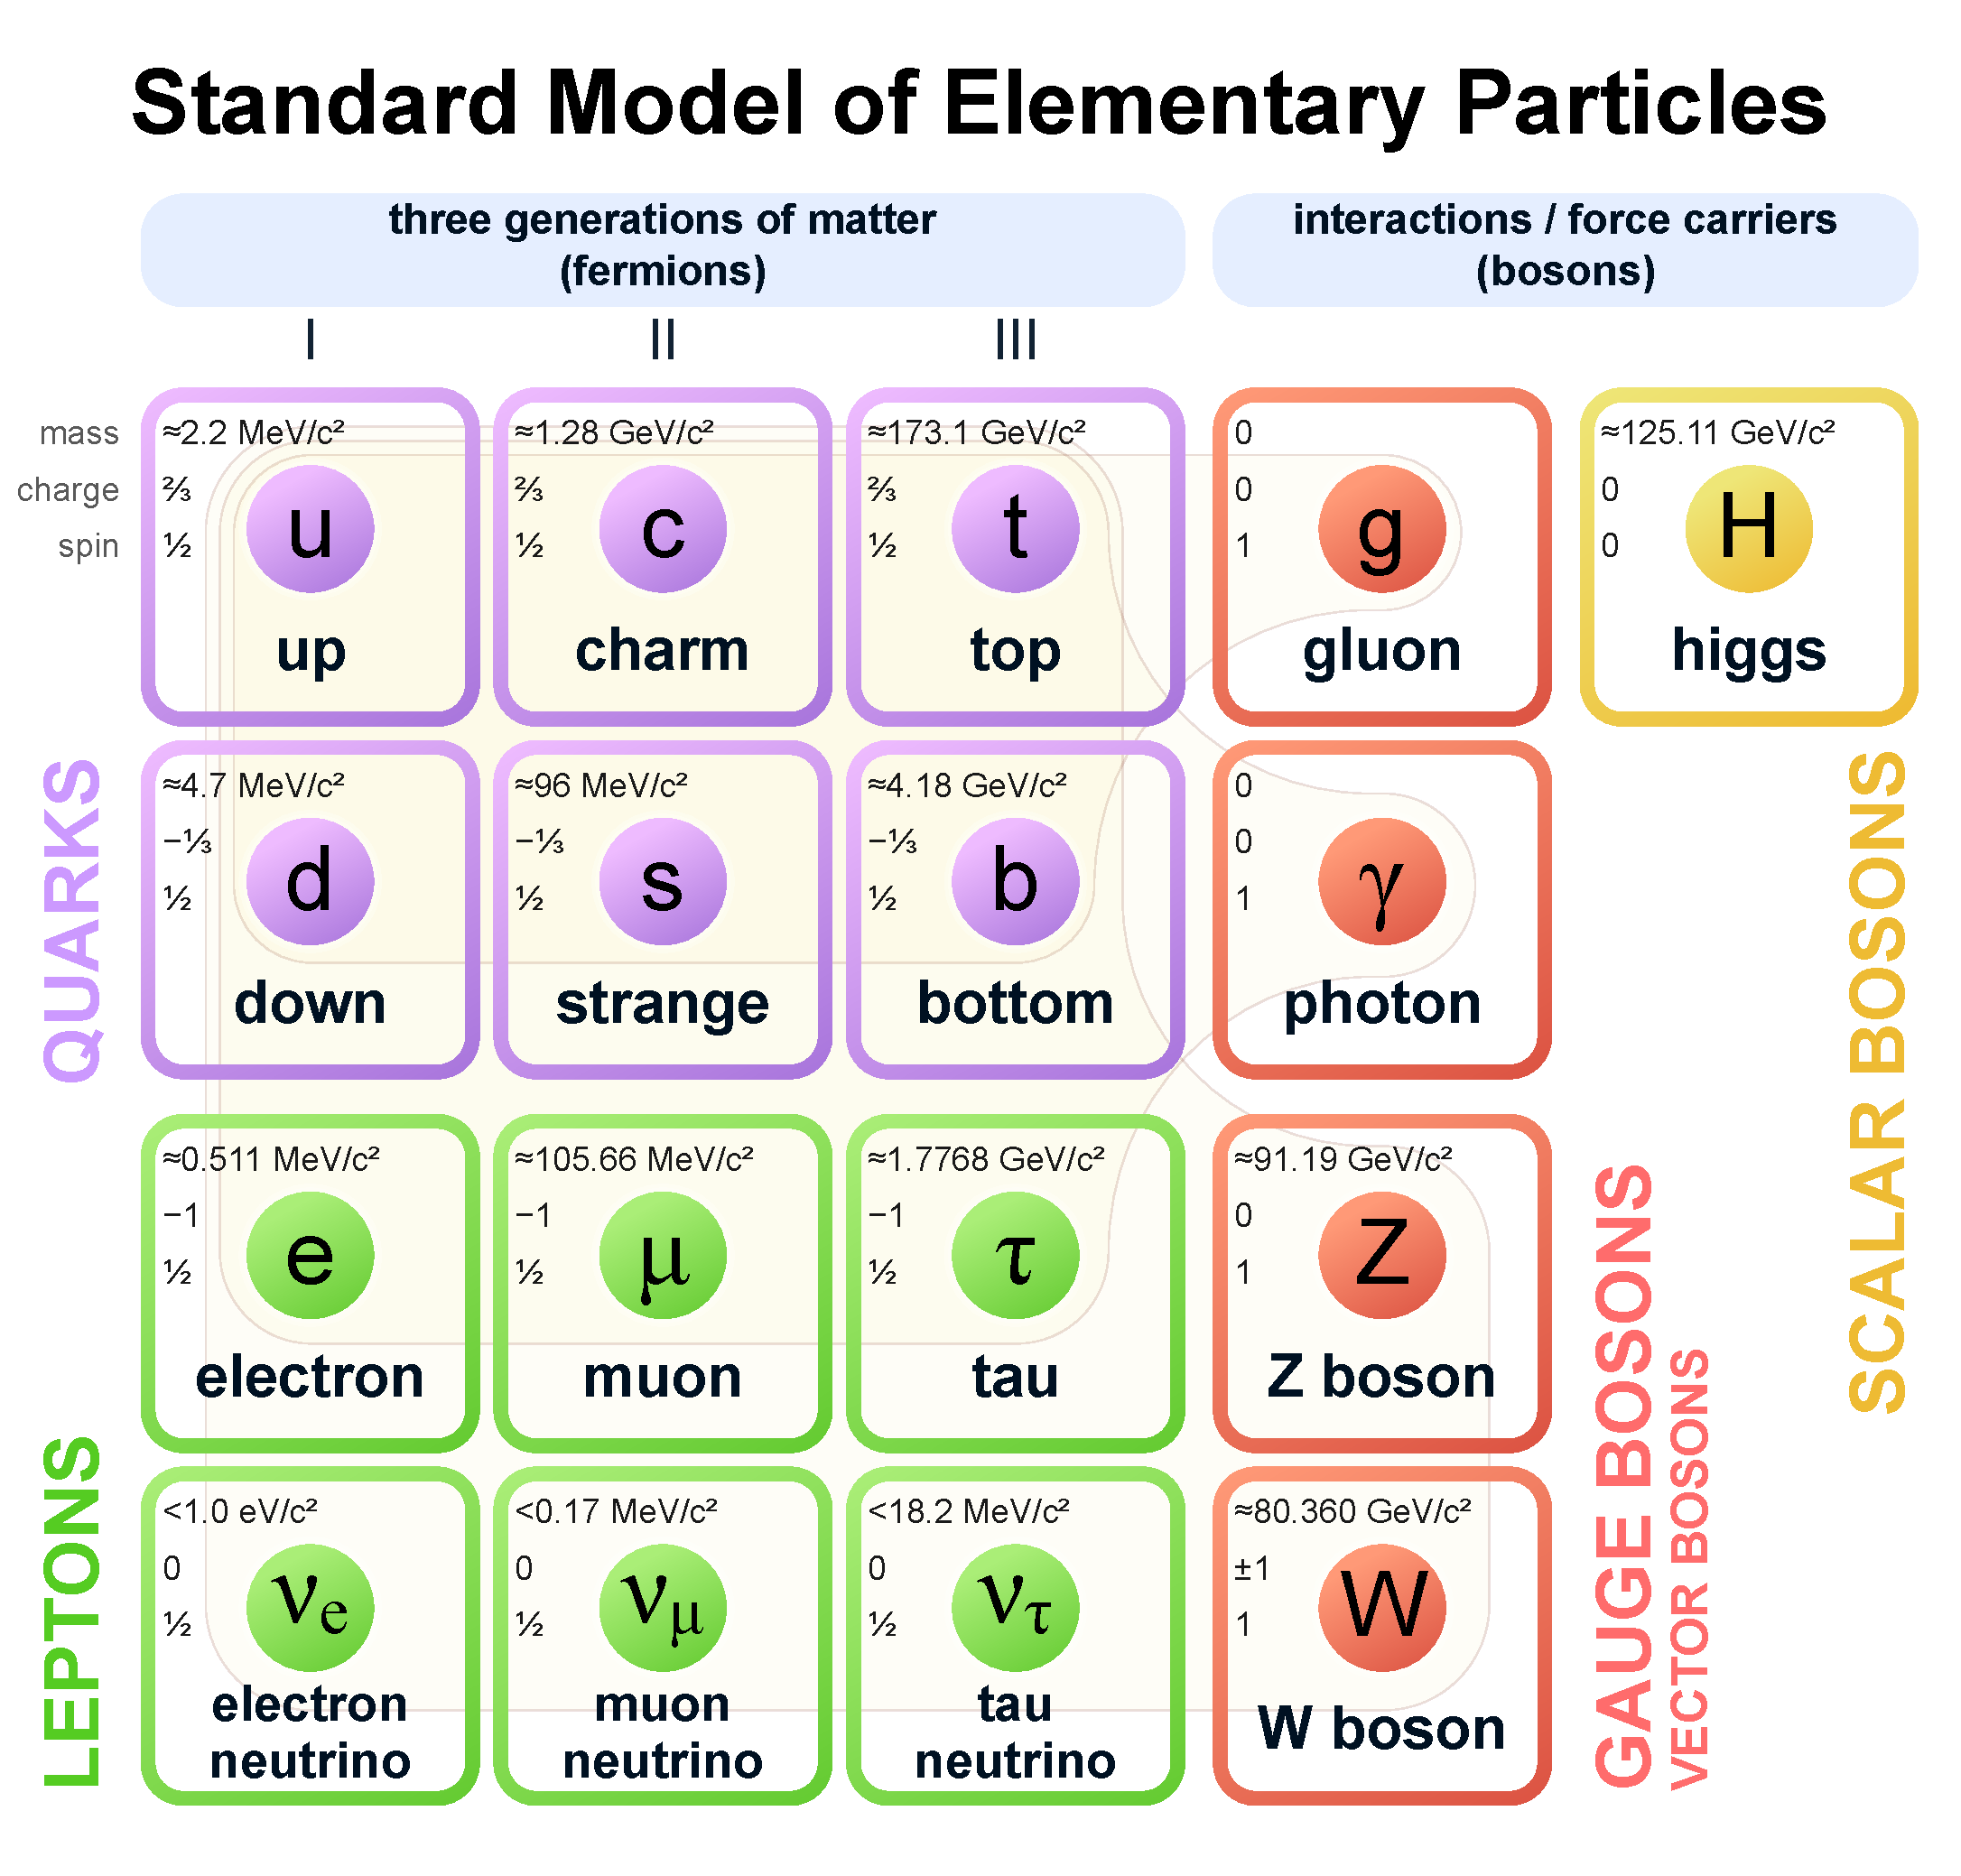
\includegraphics[width=8cm]{figures/Standard_Model_of_Elementary_Particles.pdf}
%     \caption{Table of Standard Model particles.}
%     \label{fig:intro-standard-model}
% \end{figure}



In the absence of a theoretical framework describing these particles, in the 1960s and 1970s physicists and mathematicians produced a theoretical framework called the \textbf{Standard Model (SM)} that could describe and encompass these fundamental particles and the forces that govern their interactions. The application of a mathematical theorem derived by Emmy Noether in 1918, which states that every continuous symmetry of the action of a physical system with conservative forces, has a corresponding conservation law, allowed the grouping of seventeen fundamental particles, shown in Fig. \ref{fig:intro-standard-model}.

The Standard Model groups these seventeen fundamental particles into fermions and bosons. \textbf{Fermions} consist of quarks and leptons. Quarks and leptons are grouped into three generations of matter. For example, the familiar electron falls into the first generation of leptons. The second and third generation counterparts of the electron are the muon and the tau, and are over 200 and 30,000 times heavier than the electron respectively. \textbf{Bosons} are force carriers -- in the formulation of the Standard Model, the interaction of fermions with bosons, corresponds to fundamental forces. The Standard Model describes the electromagnetic force, the strong nuclear force, and the weak nuclear force.


\subsection{The Standard Model as a gauge theory}

\subsubsection{Gauge invariance}

In this section we turn to a mathematical description of the structure of the Standard Model, specifically from the angle of gauge theories,

An example from classical physics is the electromagnetic interaction, where the fundamental field is the four-vector potential $A^\mu$. The physical electromagnetic fields and Maxwell's equations arise from the elements of the tensor $F_{\mu\nu}(x) = \partial_\mu A_\nu (x) - \partial_\nu A_\mu (x)$. Any two choices of $A^\mu$ that are related by a transformation of the form \begin{equation} A_\mu \rightarrow A_\mu + \partial_\mu \alpha \label{eqn:gauge_symmetry}\end{equation} for any real, differentiable function $\alpha(x)$, describe the same physical configuration, and has no effect on Maxwell's equations. This transformation in Eqn. \ref{eqn:gauge_symmetry} is often referred to as a \textbf{gauge symmetry}, but can also be thought of as \textbf{gauge redundancy}.


In gauge theories, the freedom of choice of gauge states that the existence and form of an interaction can be deduced from the existence of physically indeterminate, gaugable quantities.

Noether's theorem states that for every global transformation under which the Lagrangian density is invariant, there exists a conserved quantity. If $\mathcal{L}(\Psi(x), \partial_\mu \Psi(x))$ is invariant under the transformation of the wave function $\Psi(x) \rightarrow \Psi'(x)$, where $\Psi'(x) = \Psi(x) + \delta \Psi(x)$, then there exists a conserved current 
\begin{equation}
    \partial_\mu \left( \frac{\partial\mathcal{L}(x)}{\partial(\partial_\mu \Psi(x))} \delta \Psi(x)  \right) = 0
\end{equation}


\subsubsection{Local gauge symmetries}
If we modify the wave function with a phase transformation $\Psi'(x) = \exp(i e \chi) \Psi(x)$, and we allow the phase $\chi$ to be a function of spacetime, we introduce \textbf{interactions} to the theory. A wave function of the form
\begin{equation}
    \Psi'(x) = \exp(i e \chi(x)) \Psi(x)
\end{equation}
can be verified, to be not a solution to the Dirac equation for free particles: $(i \gamma^\mu \partial_\mu - m) \Psi(x) = 0$. To take the derivative of a vector field $V(x)$ (e.g. a Dirac wave function), at two displaced space-time points, in a curvilinear coordinate system, 
\begin{equation}
    \mathcal{D}_\mu \equiv \lim_{\Delta x^\mu \rightarrow 0} \frac{V_{\parallel}(x + \Delta x) - V(x)}
{\Delta x^\mu}\end{equation}

To write a derivative that is covariant under this transformation, we define a \textbf{covariant derivative}, where $A_\mu(x)$ is a 4-vector potential:
\begin{equation}
    D_\mu = \partial_\mu + i e A_\mu
\label{eqn:modified_dirac}
\end{equation}
which gives the modified Dirac equation:
\begin{equation}
    \left( i \gamma^\mu \mathcal{D}_\mu - m  \right) \Psi(x) = 0
\end{equation}
The simultaneous gauge transformation $A'_\mu(x) = A_\mu(x) - \partial_\mu\chi(x)$ and wavefunction transformation $\Psi'(x) = \exp(ie\chi(x)) \Psi(x)$ leaves the covariant-derivative form of the Dirac equation (Eqn \ref{eqn:gauge_symmetry}) invariant.

To generalize this, if the theory is invariant for unitary transformations $U$ of the particle states according to 
\begin{equation}
    \Psi' = U\Psi
\label{eqn:generic_unitary_transformation}
\end{equation}
We want to define a derivative
\begin{equation}
    D^\mu = \partial^\mu + ig B^\mu
\end{equation}
that keeps the theory invariant under Eqn. \ref{eqn:generic_unitary_transformation}. The four-potential $B^\mu$ represents the interacting four-potential which must be added to keep the theory invariant.

The Standard Model is built around the gauge transformations $G = SU(3) \times SU(2) \times U(1)$. $SU(3)$ is associated to the strong force; $SU(2)$ is associated to the weak force; and $U(1)$ is hypercharge. Electromagnetism arises from the terms $SU(2) \times U(1)$. The matter of the Standard Model (leptons and quarks, as listed in the previous section) are a regular array of fermions with fixed spacings in hypercharge quantum numbers, whose interactions enter the Lagrangian through the guage-covariant derivative:
\begin{equation}
    \mathcal{D}_\mu = \partial_\mu - ig' B_\mu \frac{Y}{2} - ig W_{\mu}^{\alpha} \frac{\tau_a}{2} - ig_s G_\mu^{k} \frac{\lambda_k}{2}
\end{equation}

\subsection{The Higgs Mechanism}
Local gauge invariance of the Standard Model Lagrangian under $SU(3)_C \times SU(2)_L \times U(1)_Y$ requires massless fermions and massless force carriers of the interaction. However, if the physical vacuum does not have all the symmetries of the Lagrangian, then the propagation of the gauge particles and all the fermions is modified. The symmetries of the physical vacuum must be spontaneously broken, without affecting gauge invariance in the Lagrangian. 

The \textbf{Higgs mechanism} proposes the existence of a scalar field, or fields, with nonzero vacuum expectation values, which reduce the gauge symmetries of the physical vacuum from $SU(3)_C \times SU(2)_L \times U(1)_Y$ down to $SU(3)_C \times U(1)_{EM}$. The Higgs field interacts with the gauge bosons and fermions throughout space, impeding their free propagation. The resulting broken symmetry correctly predicts the mass ratio of the neutral (Z) and charged (W) massive electroweak bosons, and predicts that at least one physical degree of freedom in the Higgs field is a particle degree of freedom, called the \textbf{Higgs boson}. The location of the minimum of the Higgs potential can be constrained from previously measured Standard Model parameters, but the shape of the mass distribution of the Higgs boson must be experimentally measured.

The \textit{minimal choice of Higgs field} comes from the breaking of $SU(2)_L \times U(1)_Y$ down to $U(1)_{EM}$. The smallest $SU(2)$ multiplet is the doublet. The existence of three massive electroweak bosons leads the Higgs sector to have at least three degrees of freedom. The minimal single-doublet complex scalar Higgs field is
\begin{equation}
    \Phi(x) = \begin{pmatrix} \phi^+(x) \\ \phi^0(x) \end{pmatrix} 
    = \frac{1}{\sqrt{2}} \begin{pmatrix} \phi_1^+(x) + i\phi_2^+(x) \\ \phi_1^0(x) + i\phi_2^0 (x) \end{pmatrix}
\end{equation}
where $\phi_1^+$, $\phi_2^+$, $\phi_1^0$, and $\phi_2^0$ are real (four degrees of freedom). By convention, the nonzero vacuum expectation value is assigned to $\phi_1^0$.

The minimal self-interacting Higgs potential that is invariant under $SU(2)_L \times U(1)_Y$ is given by
\begin{equation}
    V(\Phi^\dagger \Phi) = -\mu^2 \Phi^\dagger \Phi + \lambda (\Phi^\dagger \Phi)^2, \,\,\, \mu^2 > 0, \, \lambda > 0
\end{equation}
where $\lambda$ is the coupling strength of the four-point Higgs interaction. 
The potential energy is minimized at 
\begin{equation}
    \Phi_{\text{min}} = \frac{1}{\sqrt{2}} \begin{pmatrix} 0 \\ v \end{pmatrix}, \,\,\,\text{where} \, v = \sqrt{\mu^2 / \lambda}
\end{equation}
Choosing a fixed orientation of $\langle \Phi \rangle$ out of a continuous set of possible ground states spontaneously breaks the symmetry of the physical vacuum.

The excitations of the Higgs field with respect to the minimum $\Phi_{\text{min}}$ are parametrized by 
\begin{equation}
    \Phi(x) = \exp(i \boldsymbol{\xi}(x) \cdot \boldsymbol{\tau}) \frac{1}{\sqrt{2}} \begin{pmatrix} 0 \\ v + H(x) \end{pmatrix}
\end{equation}
Three degrees of freedom are coupled directly to the electroweak gauge bosons; this is often referred to as the gauge bosons ``eating up'' the Goldstone bosons to form the longitudinal polarizations of the massive spin-1 boson states. The $H(x)$ excitation is in the radial direction and corresponds to the free particle state of the Higgs boson. 

\subsection{Two-Higgs Doublet Models}

% https://www.damtp.cam.ac.uk/user/tong/sm/standardmodel1.pdf
 
\section{Sources}

    \begin{itemize}
        \item \texttt{https://www.space.com/standard-model-physics}
        \item \texttt{https://www.iop.org/explore-physics/big-ideas-physics/standard-model}
        \item Wikipedia
        \item \texttt{https://www.damtp.cam.ac.uk/user/tong/sm/standardmodel1.pdf}
    \end{itemize}

\end{document}